\documentclass[a4paper,utf8]{article}
\usepackage{rapport}
\usepackage[normalem]{ulem}
\usepackage{amsfonts}
\usepackage{graphicx}
\usepackage{MnSymbol,wasysym}
\usepackage{hyperref}
\usepackage[french]{babel}


\formation{L3MI}
\date{}
\matiere{Conception Orient�e Objet}
\titre{Bataille Navale - Compte Rendu}

\newcommand\code[1]{\textsf{#1}}
\newcommand\srdjan[1]{{\color{red} #1}}

\begin{document}

\entete

\section{Ce qui a �t� r�alis�}

-Impl�mentation du jeu Bataille Navale en r�seau.\\%
-Cr�ation d'un serveur r�alisant la liaison entre deux clients.\\%
-Possibilit� de choisir son port.\\%


\section{Difficult�s rencontr�es : gestion des erreurs de communication}


Afin de r�aliser les communications, on a cr�� un serveur et deux clients.\\%

\begin{itemize}

    \item \textbf{Au niveau du serveur:}\\% 
    Apr�s avoir indiqu� le port, on initialise deux threads "AccepterClients", qui attendent la connexion de deux clients simultan�s, pour ensuite confirmer le d�marrage de la partie.
    \item \textbf{Au niveau du client:}\\%
    A la cr�ation du client, on tente la connexion au serveur. Si la connexion est r�ussie, on lance le thread "RecevoirInfos" qui r�cup�re l'ensemble des messages envoy�s par le serveur et les traitent.
	\item \textbf{Au niveau de la vue (cot� client):}\\% 
	En fonction des �v�nements souris, on va envoyer des messages au serveur. Celui-ci va faire la passerelle et l'envoyer au second client (qui va r�cup�rer le message sur "RecevoirInfos").

\end{itemize}


\newpage


\section{Description du protocole r�seau}

Quelques modifications ont �t� apport� sur le protocole initialement d�crit dans le sujet, ceci �tant du au fait que le serveur n'est pas un client.\\%

Ci-dessous, une description du protocole:

\makebox[\textwidth]{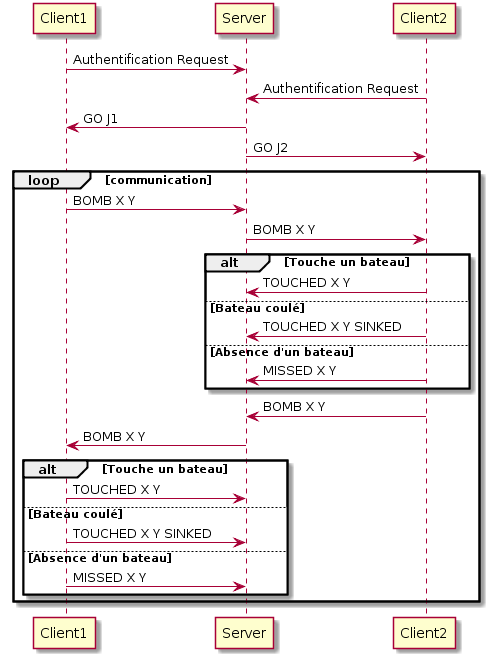
\includegraphics[width=300pt]{img/diag}}



\end{document}